%%
%% This is file `sample-sigconf-biblatex.tex',
%% generated with the docstrip utility.
%%
%% The original source files were:
%%
%% samples.dtx  (with options: `all,proceedings,sigconf-biblatex')
%%
%% IMPORTANT NOTICE:
%%
%% For the copyright see the source file.
%%
%% Any modified versions of this file must be renamed
%% with new filenames distinct from sample-sigconf-biblatex.tex.
%%
%% For distribution of the original source see the terms
%% for copying and modification in the file samples.dtx.
%%
%% This generated file may be distributed as long as the
%% original source files, as listed above, are part of the
%% same distribution. (The sources need not necessarily be
%% in the same archive or directory.)
%%
%%
%% Commands for TeXCount
%TC:macro \cite [option:text,text]
%TC:macro \citep [option:text,text]
%TC:macro \citet [option:text,text]
%TC:envir table 0 1
%TC:envir table* 0 1
%TC:envir tabular [ignore] word
%TC:envir displaymath 0 word
%TC:envir math 0 word
%TC:envir comment 0 0
%%
%% The first command in your LaTeX source must be the \documentclass
%% command.
%%
%% For submission and review of your manuscript please change the
%% command to \documentclass[manuscript, screen, review]{acmart}.
%%
%% When submitting camera ready or to TAPS, please change the command
%% to \documentclass[sigconf]{acmart} or whichever template is required
%% for your publication.
%%
%%
\documentclass[sigconf,natbib=false]{acmart}
%%
%% \BibTeX command to typeset BibTeX logo in the docs
\AtBeginDocument{%
  \providecommand\BibTeX{{%
    Bib\TeX}}}

%% Rights management information.  This information is sent to you
%% when you complete the rights form.  These commands have SAMPLE
%% values in them; it is your responsibility as an author to replace
%% the commands and values with those provided to you when you
%% complete the rights form.
\setcopyright{acmlicensed}
\copyrightyear{2025}
\acmYear{2025}
\acmDOI{}
%% These commands are for a PROCEEDINGS abstract or paper.
\acmConference[]{Artificial Intelligence Foundation Assignment}{2025}{NeoSchool}
%%
%%  Uncomment \acmBooktitle if the title of the proceedings is different
%%  from ``Proceedings of ...''!
%%
%%\acmBooktitle{Woodstock '18: ACM Symposium on Neural Gaze Detection,
%%  June 03--05, 2018, Woodstock, NY}
\acmISBN{}


%%
%% Submission ID.
%% Use this when submitting an article to a sponsored event. You'll
%% receive a unique submission ID from the organizers
%% of the event, and this ID should be used as the parameter to this command.
%%\acmSubmissionID{123-A56-BU3}

%%
%% For managing citations, it is recommended to use bibliography
%% files in BibTeX format.
%%
%% You can then either use BibTeX with the ACM-Reference-Format style,
%% or BibLaTeX with the acmnumeric or acmauthoryear sytles, that include
%% support for advanced citation of software artefact from the
%% biblatex-software package, also separately available on CTAN.
%%
%% Look at the sample-*-biblatex.tex files for templates showcasing
%% the biblatex styles.
%%


%%
%% The majority of ACM publications use numbered citations and
%% references, obtained by selecting the acmnumeric BibLaTeX style.
%% The acmauthoryear BibLaTeX style switches to the "author year" style.
%%
%% If you are preparing content for an event
%% sponsored by ACM SIGGRAPH, you must use the acmauthoryear style of
%% citations and references.
%%
%% Bibliography style
\RequirePackage[
  datamodel=acmdatamodel,
  style=acmnumeric,
  ]{biblatex}

%% Declare bibliography sources (one \addbibresource command per source)
\addbibresource{software.bib}
\addbibresource{sample-base.bib}

%%
%% end of the preamble, start of the body of the document source.
\begin{document}

%%
%% The "title" command has an optional parameter,
%% allowing the author to define a "short title" to be used in page headers.
\title{Overview of Diffusion Models}

%%
%% The "author" command and its associated commands are used to define
%% the authors and their affiliations.
%% Of note is the shared affiliation of the first two authors, and the
%% "authornote" and "authornotemark" commands
%% used to denote shared contribution to the research.
\author{Harry Huang}
\email{harryhuang2652@qq.com}
\affiliation{%
  \institution{University of Science and Technology Beijing}
  \city{Beijing}
  \country{China}
}

%%
%% The abstract is a short summary of the work to be presented in the
%% article.
\begin{abstract}
  Diffusion models have emerged as a powerful class of generative models,
  offering high-quality data generation through a gradual noising and denoising process.
  This paper provides a comprehensive review of the key concepts and advancements in diffusion models,
  including Diffusion Probabilistic Models (DPMs), Denoising Diffusion Probabilistic Models (DDPMs),
  and Noise Conditional Score Networks (NCSNs).
  We discuss their applications in computer vision, natural language processing, and time series forecasting,
  as well as the challenges related to computational efficiency and generation quality.
  Finally, we outline potential future directions for improving these models.
\end{abstract}

%%
%% Keywords. The author(s) should pick words that accurately describe
%% the work being presented. Separate the keywords with commas.
\keywords{Diffusion Model, Generative AI, Image Generation}

%%
%% This command processes the author and affiliation and title
%% information and builds the first part of the formatted document.
\maketitle

\section{Introduction}
Before the invention of diffusion models,
Generative Adversarial Networks (GANs) and Variational Autoencoders (VAEs)
were the dominant generative models.

GANs achieve data generation by training two adversarial models:
a discriminator (D) and a generator (G).
The discriminator aims to distinguish between real data and data generated by the generator,
while the generator aims to produce data that can "fool" the discriminator.
Through this adversarial learning mechanism, GANs can generate highly realistic data.
However, GAN training is often unstable,
prone to issues such as mode collapse and vanishing gradients. \cite{weng2018}

In contrast, VAEs learn latent representations of data by optimizing a variational lower bound.
Although VAEs offer more stable training,
the quality of generated samples is generally inferior to that of GANs. \cite{goodfellow2014}

The invention of diffusion models has brought new breakthroughs
to the field of generative modeling.
By defining forward noising and reverse denoising processes,
diffusion models combine the high-quality generation capability of GANs
with the training stability of VAEs.

\section{Basic Ideas}
As mentioned in the introduction, the whole process of diffusion models can be divided
into two parts: forward noising and backward denoising. \cite{sohldickstein2015} \cite{ho2020}

\subsection{Forward Noising}
given a real data distribution \( x_0 \),
we gradually add Gaussian noise to the data distribution over \( T \) steps,
eventually obtaining the noised data distribution \( x_T \).
Clearly, when \( T \) reaches a certain level, the features of \( x_T \) become indistinguishable,
eventually converging to a true isotropic Gaussian distribution.

Specifically, the forward diffusion process can be expressed as:
\[
x_t = \sqrt{\alpha_t} x_{t-1} + \sqrt{1 - \alpha_t} \epsilon_t, \quad \epsilon_t \sim \mathcal{N}(0, I)
\]
where \( \alpha_t \) is the noise scheduling parameter at step \( t \),
and \( \epsilon_t \) is noise sampled from a standard Gaussian distribution.

\subsection{Backward Denoising}

In the reverse denoising stage,
we need to gradually remove noise from an isotropic Gaussian noise map \( x_T \)
to try to restore it to the original image \( x_0 \).
To estimate the conditional distribution \( q(x_{t-1} \mid x_t) \) in the denoising stage,
we employ machine learning techniques to learn a parameterized model
\( p_\theta \) from a large amount of data.
By learning \( p_\theta \), the model can approximate the reverse diffusion process,
enabling step-by-step reconstruction from noise to data.

Specifically, the model aims to minimize the following objective function:
\[
{L}(\theta) = \mathbb{E}_{x_0, \epsilon, t} \left[ \| \epsilon - \epsilon_\theta(x_t, t) \|^2 \right]
\]
where \( \epsilon_\theta(x_t, t) \) is the noise predicted by the model, \( \epsilon \) is the actual noise added, and \( t \) is the timestep. By optimizing this objective, the model gradually learns how to recover the original data from noise.

\section{Models Overview}

\subsection{Diffusion Probabilistic Models}
Diffusion Probabilistic Models (DPMs) are a class of generative models
that model the data generation process as a Markov chain of stochastic diffusion steps.
The process involves a forward diffusion that gradually adds noise to the data,
transforming it into a simple noise distribution,
and a learned reverse diffusion process that removes the noise to generate new data samples.

\begin{figure}[h]
  \centering
  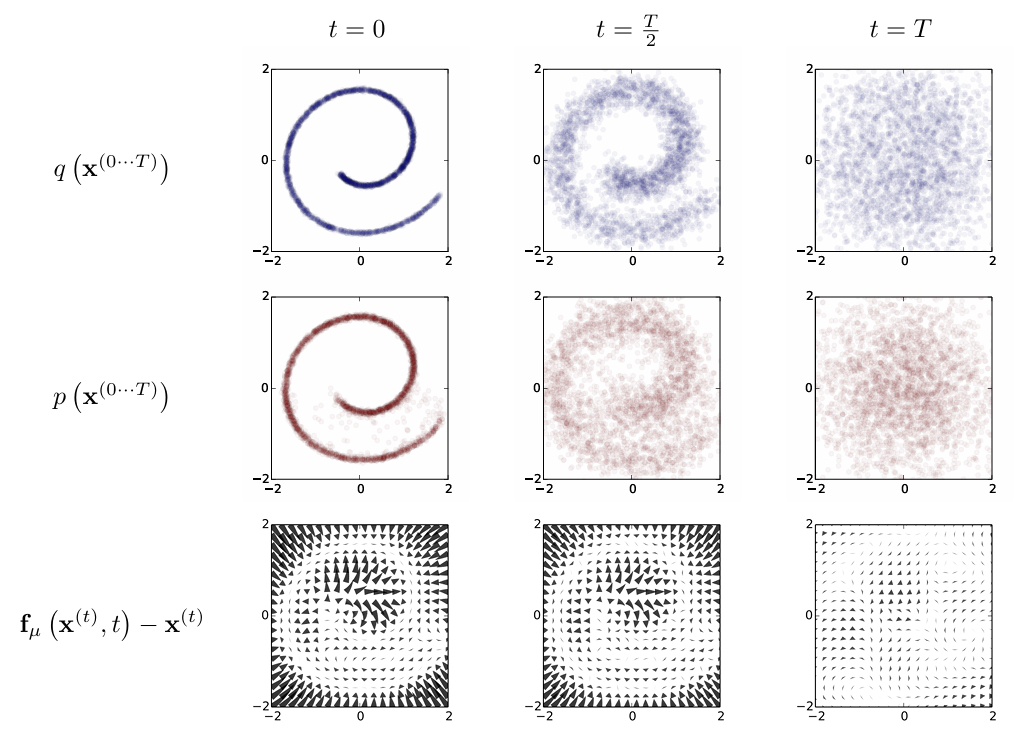
\includegraphics[width=\linewidth]{imgs/150303585-F1.png}
  \caption{Illustration shows a modeling framework trained on 2D swiss roll data.
  Image source: \cite[Sohl-Dickstein et al. (2015)]{sohldickstein2015}.}
  \Description{}
\end{figure}

The forward diffusion process is defined as a sequence of conditional distributions:
\[
q(x_t | x_{t-1}) = \mathcal{N}(x_t; \sqrt{1 - \beta_t} x_{t-1}, \beta_t I),
\]
where \(\beta_t\) is a variance schedule that controls the amount of noise added at each timestep \(t\).

The reverse process is learned and is defined as:
\[
p_\theta(x_{t-1} | x_t) = \mathcal{N}(x_{t-1}; \mu_\theta(x_t, t), \sigma_\theta(x_t, t)),
\]
where \(\mu_\theta\) and \(\sigma_\theta\) are typically parameterized by neural networks.

\begin{figure}[h]
  \centering
  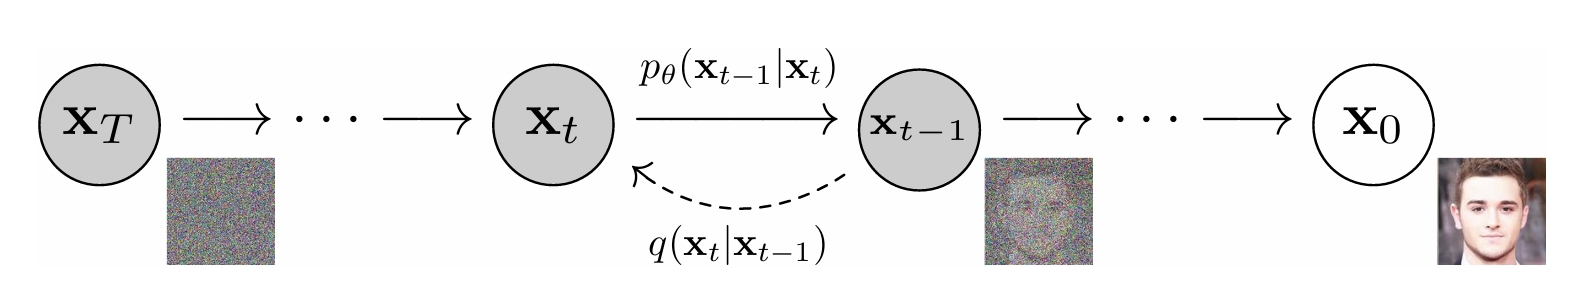
\includegraphics[width=\linewidth]{imgs/200611239-F2.png}
  \caption{Illustration shows the basic forward and backward process in DPMs.
  Image source: \cite[Ho et al. (2020)]{ho2020}.}
  \Description{}
\end{figure}

\textbf{Training Objective:}

In Diffusion Probabilistic Models (DPMs),
the goal is to learn a generative model by defining a forward diffusion process
that gradually adds noise to the data, transforming it into a simple noise distribution.
The training objective in DPMs is to minimize the discrepancy
between the learned reverse process and the true reverse process.

This is typically achieved by optimizing a loss function
that measures the difference between the two processes,
often using variational inference techniques to approximate the true reverse process.
We will see a detailed and better implementation in DDPM section,
while DPM is more likely a abstract framework.

\textbf{Comparison to GANs and VAEs:}

Generative Adversarial Networks (GANs) excel at generating sharp images
but suffer from mode collapse and lack a direct way to compute likelihoods.
Variational Autoencoders (VAEs) provide an explicit likelihood model
but often struggle with posterior collapse and may generate blurry samples.

DPMs, on the other hand, offer a balance by providing a tractable likelihood
and generating high-quality samples,
albeit with higher computational costs during training and sampling.
Also, they can handle a variety of data types and have flexible model architectures.
They also connect to variational inference and Langevin dynamics,
providing a rich theoretical foundation. \cite{welling2011}

\begin{figure}[h]
  \centering
  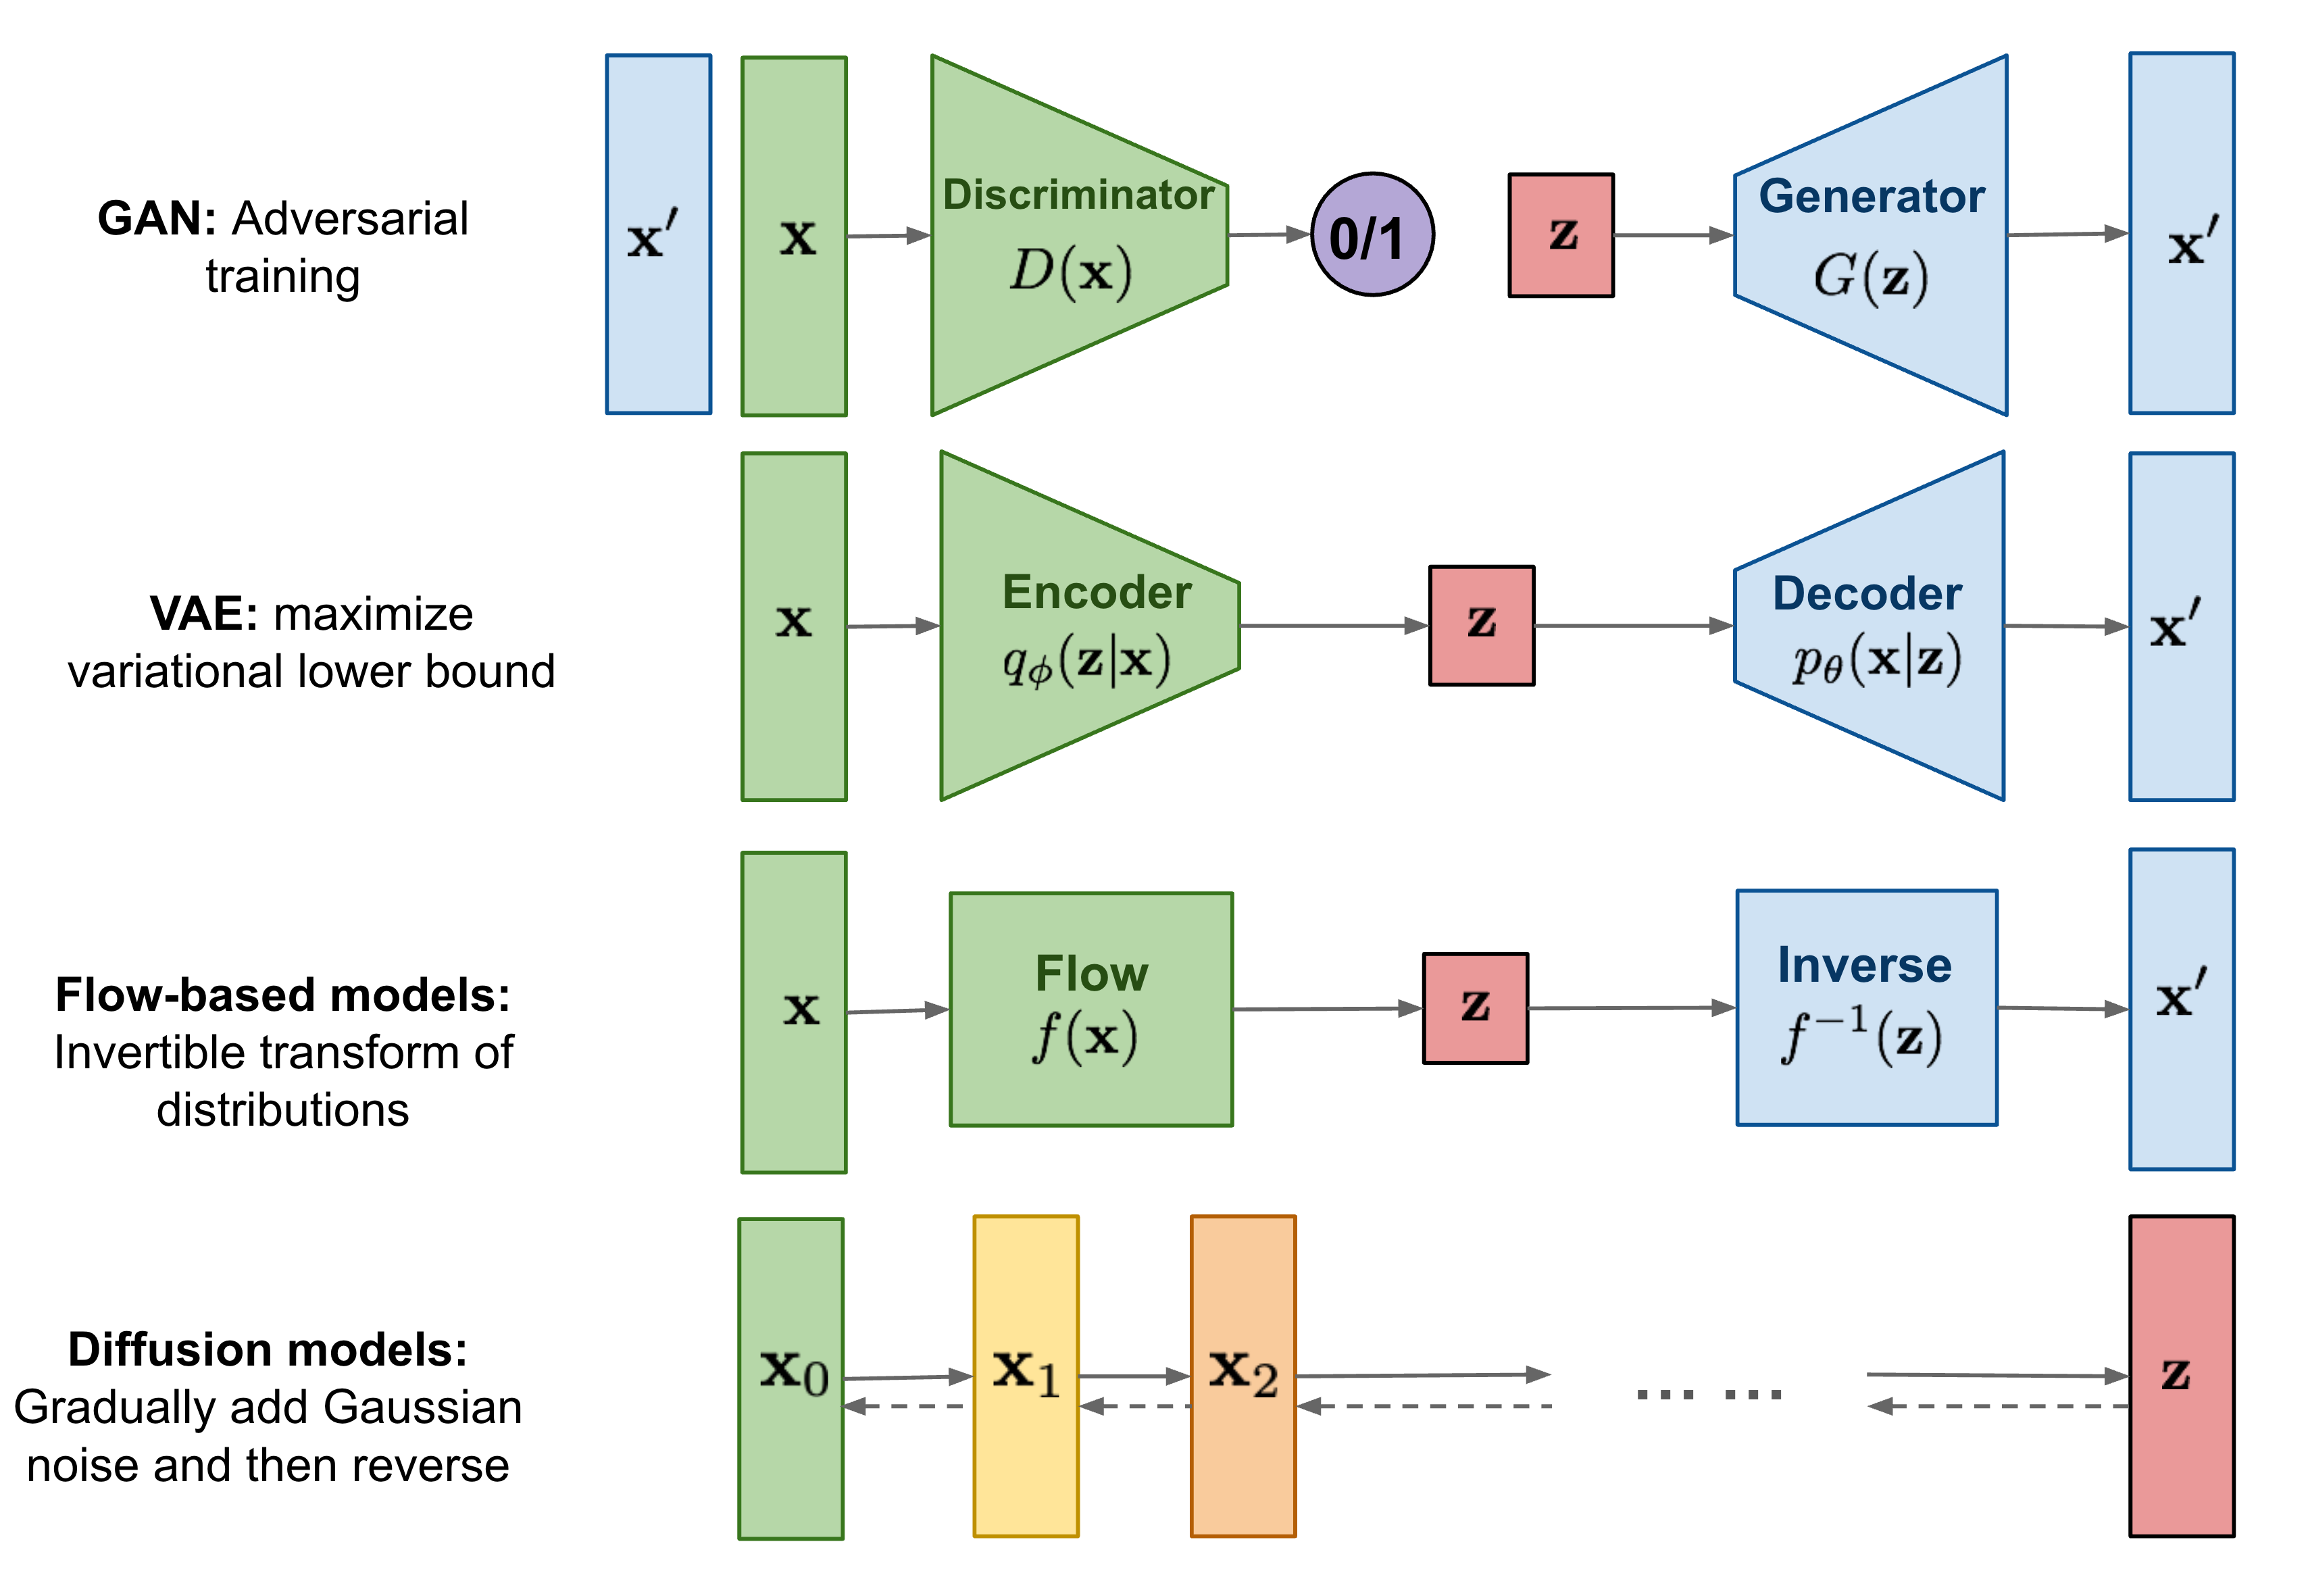
\includegraphics[width=\linewidth]{imgs/lilianweng2107-F1.png}
  \caption{Illustration shows the different types of diffusion models.
  Image source: \cite[Weng (2021)]{weng2021}.}
  \Description{}
\end{figure}

\subsection{Denoising Diffusion Probabilistic Models}
Denoising Diffusion Probabilistic Models (DDPMs) are a specialized class
of Diffusion Probabilistic Models (DPMs) designed for high-quality image generation.
DDPMs focus on the denoising aspect of the diffusion process,
utilizing a discrete-time formulation to model the data generation process.

\textbf{Training Objective:}

DDPMs optimize a specific Evidence Lower Bound (ELBO) derived from the data likelihood.
The training objective is to minimize the mean squared error
between the added noise \(\epsilon\) and the predicted noise \(\epsilon_\theta(x_t, t)\):
\[
\mathcal{L}(\theta) = \mathbb{E}_{x_0, \epsilon, t} \left[ \left\| \epsilon - \epsilon_\theta(x_t, t) \right\|^2 \right],
\]
where \(x_t = \sqrt{\bar{\alpha}_t} x_0 + \sqrt{1 - \bar{\alpha}_t} \epsilon\),
and \(\alpha_t = 1 - \beta_t\), \(\bar{\alpha}_t = \prod_{s=1}^t \alpha_s\).

DDPMs significantly contribute to the field of DPMs by offering a practical
and efficient implementation for image generation tasks,
demonstrating the potential of diffusion models for high-quality data synthesis.

\textbf{Progressive Lossy Decompression:}

DDPMs employ a progressive lossy decompression mechanism,
where the model iteratively refines the data by removing noise at each timestep.
This process can be seen as a form of autoregressive generation,
where each step depends on the previous one, leading to high-fidelity sample reconstruction.

\subsection{Noise Conditional Score Network}
Noise Conditional Score Networks (NCSNs) are a sophisticated approach
within score-based generative modeling,
designed to estimate the score function of data perturbed with varying noise levels.

NCSNs are a class of models that estimate the score function,
which is the gradient of the log probability density,
for data points corrupted with Gaussian noise at multiple scales.
This estimation is crucial for performing Langevin dynamics to generate new samples.

Score matching is a technique used to train models to estimate the score function.
It is advantageous for generative modeling as it directly targets the gradient
of the data distribution, facilitating the learning of complex structures.

The manifold hypothesis posits that real data lies on a low-dimensional manifold
within a high-dimensional space.
NCSNs address the challenges posed by this hypothesis by perturbing data
with Gaussian noise at various scales,
thereby robustly estimating the score function near the data manifold.

Noise conditioning in NCSNs involves conditioning the score estimation on the noise level or scale.
This allows the model to adapt its score estimates
based on the noise structure at different levels, enhancing estimation accuracy.

\textbf{Training Objective:}

NCSNs are trained to minimize the mean squared error between the true score
and the estimated score at different noise levels.
The training loss function is:
\[ \mathcal{L}(\theta) = \mathbb{E}_{x, \epsilon, \sigma} \left[ \| s(x + \sigma \epsilon) - s_\theta(x + \sigma \epsilon, \sigma) \|^2 \right] \]
where \( s(x) = \nabla \log p(x) \) is the true score,
and \( s_\theta \) is the estimated score.

\textbf{Sampling Process:}

Annealed Langevin dynamics is a sampling technique that involves gradually
reducing the noise level during the sampling process.
This method guides the samples from the prior distribution towards the data distribution,
ensuring a smooth transition.

The sampling process in NCSNs involves iteratively updating the samples
using annealed Langevin dynamics:
\[ x_{k+1} = x_k + \frac{\eta}{2} s_\theta(x_k, \sigma_k) + \sqrt{\eta} \cdot \epsilon_k \]
where \(\eta\) is the step size,
\(\sigma_k\) is the noise scale at step \(k\), and \(\epsilon_k \sim \mathcal{N}(0, I)\).

After all, NCSNs offer several advantages,
including robust score estimation and flexible sampling mechanisms.

\section{Applications and Impact}
Diffusion Probabilistic Models (DPMs), Denoising Diffusion Probabilistic Models (DDPMs),
and Noise Conditional Score Networks (NCSNs)
have emerged as significant breakthroughs in the field of generative modeling,
demonstrating exceptional performance and broad influence across various practical applications.

These models have achieved remarkable results not only in computer vision tasks
such as image generation and restoration
but also shown great potential in natural language processing (NLP)
and time series forecasting.

\subsection{Computer Vison}
In computer vision, these models have excelled in tasks such as image generation,
restoration, and enhancement.

DDPM, with its high-quality image generation capabilities,
has achieved performance comparable to or even superior to GANs on benchmark datasets
like CIFAR-10 and LSUN \cite{ho2020}.
Additionally, NCSN, through multi-scale noise perturbation and annealed Langevin dynamics,
has demonstrated powerful representation learning capabilities
in image restoration and denoising tasks.

The efficiency and flexibility of these models make them highly valuable
in practical applications such as medical image processing and satellite image analysis.

\subsection{Natural Language Processing}
In NLP, diffusion models and score matching methods have provided new approaches
for text generation and language modeling. \cite{li2022}

While traditional autoregressive models (e.g., GPT series) have achieved significant success,
they face limitations in long-text generation and diversity control.
Diffusion models, with their non-autoregressive nature,
enable parallel generation of high-quality text, significantly improving generation efficiency.

Moreover, score matching-based methods have shown potential in text denoising and restoration tasks,
such as machine translation and text summarization.

\subsection{Time Series Forecasting}
In time series forecasting, these models have offered new solutions for tasks in finance,
meteorology, and healthcare through their powerful probabilistic modeling capabilities. \cite{tashiro2021}

Diffusion models can effectively capture complex dependencies
and nonlinear dynamics in time series data,
excelling in tasks such as stock price prediction, weather forecasting,
and disease spread prediction.

Compared to traditional methods like ARIMA and RNNs,
diffusion models exhibit clear advantages in handling high-dimensional and non-stationary data.

\section{Challenges and Limitations}
Despite the significant progress of diffusion models
in the field of generative modeling and their demonstrated potential in tasks
such as image generation, text synthesis, and time series forecasting,
they still face several challenges and limitations in practical applications.
These challenges are discussed below from two perspectives:
computational efficiency and generation quality.

\subsection{Computational Efficiency}
A major challenge of diffusion models is their high computational cost.
Since the diffusion process typically requires hundreds or even thousands of sampling steps,
the speed of sample generation is much slower compared to other generative models.

For example, \cite[Song et al. (2022)]{song2022}
noted that generating 50k images of size 32×32 takes about 20 hours,
whereas GANs can achieve this in less than a minute.
This limits the practicality of diffusion models in real-time applications
and large-scale data generation.

\textbf{Improvement directions:}
\begin{itemize}
  \item \textbf{Reducing Sampling Steps}:
  Strided sampling schedules \cite[Nichol \& Dhariwal (2021)]{nichol2021}
  and Denoising Diffusion Implicit Models \cite[DDIM; Song et al. (2022)]{song2022}
  significantly reduce the number of sampling steps while maintaining generation quality.
  \item \textbf{Progressive Distillation}:
  \cite[Salimans \& Ho (2022)]{salimans2022} proposed progressive distillation,
  which distills a trained diffusion model into a model with fewer steps,
  gradually reducing sampling complexity.
  \item \textbf{Consistency Models}:
  \cite[Song et al. (2023)]{song2023} introduced consistency models,
  which directly map noisy data points to their origins,
  enabling single-step generation and greatly improving efficiency.
  \begin{figure}[h]
    \centering
    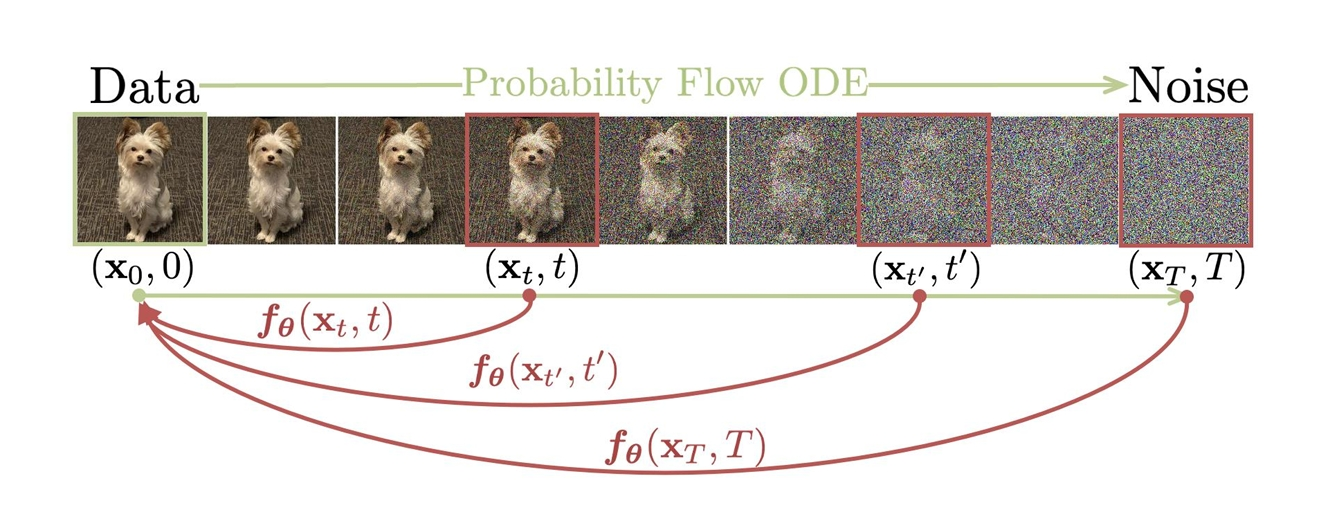
\includegraphics[width=\linewidth]{imgs/230301469-F1.png}
    \caption{Illustration shows consistency models learn to map any data point on the trajectory back to origin.
    Image source: \cite[Song et al. (2023)]{song2023}.}
    \Description{}
  \end{figure}
\end{itemize}

\subsection{Generation Quality}
Diffusion models still face limitations in certain tasks.
For instance, the generation quality of DDPM significantly degrades
when the number of sampling steps is small \cite[Song et al. (2022)]{song2022}.
Additionally, the ability of diffusion models to generate fine details
in high-resolution images needs further improvement.

\textbf{Improvement directions:}
\begin{itemize}
  \item \textbf{Latent Diffusion Models (LDM)}:
  \cite[Rombach \& Blattmann et al. (2022)]{rombach2022}
  proposed performing the diffusion process in a latent space,
  reducing computational complexity while maintaining generation quality.
  \item \textbf{Cascaded Diffusion Models}:
  \cite[Ho et al. (2021)]{ho2021} introduced cascaded diffusion models,
  which generate high-resolution images progressively through multiple resolutions,
  significantly enhancing detail generation.
  \begin{figure}[h]
    \centering
    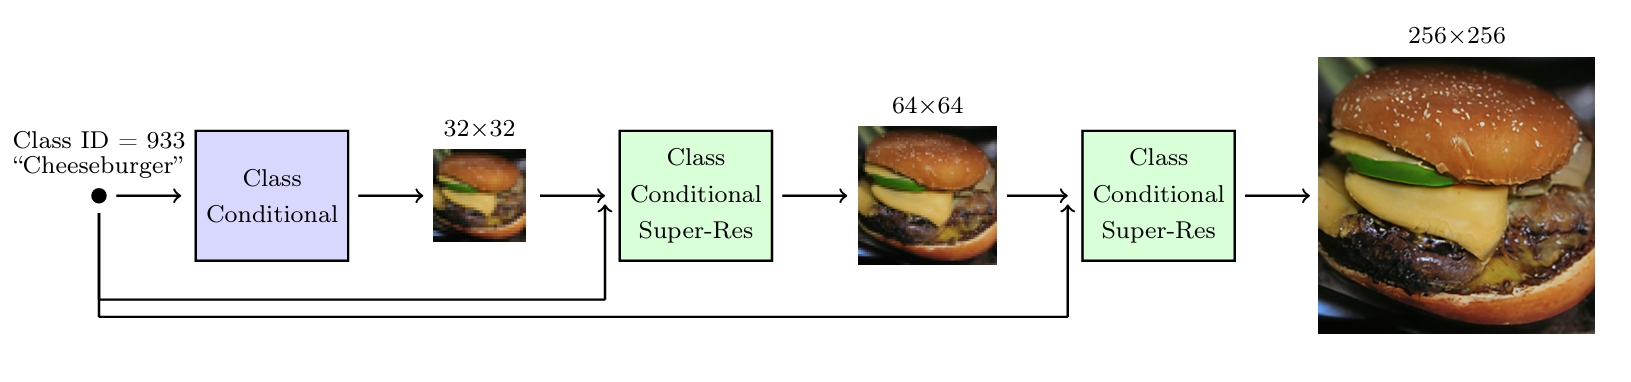
\includegraphics[width=\linewidth]{imgs/210615282-F4.png}
    \caption{Illustration shows a cascaded diffusion model generating a class-specified image.
    Image source: \cite[Ho et al. (2021)]{ho2021}.}
    \Description{}
  \end{figure}
  \item \textbf{Noise Conditioning Augmentation}:
  Introducing noise conditioning augmentation during training reduces error accumulation
  in cascaded models, further improving generation quality.
\end{itemize}

\section{Conclusion}
Diffusion models have revolutionized the field of generative modeling,
providing a unique combination of high-quality generation and training stability.
Despite their success, challenges related to computational efficiency and generation quality remain.
Future research directions may include further optimization of sampling algorithms,
exploration of new architectures, and application of diffusion models to emerging domains
such as reinforcement learning and multimodal data generation.

%%
%% Print the bibliography
%%
\printbibliography

\end{document}
\endinput
%%
%% End of file `sample-sigconf-biblatex.tex'.
